\subsubsection{Общая структура проектного решения}
Глобально проект состоит из двух компонент. Первая отвечает за интерактивное
взаимодействие с пользователем и генерацию кода второй компоненты с
использованием указанных пользователем алгоритмов (далее --- компоновщик).
Вторая --- это имплементация блокчейна (далее --- реализация блокчейна).
Проект содержит код для кошелька ({\small wallet.py}) и майнера ({\small
miner.py}) с определённой функциональностью. Код второго проекта структурирован
для удовлетворения нужд использования указанных пользователем методов. Методы и
классы генерируются at-runtime первого приложения.

\paragraph{Язык программирования}
Использованный язык программирования --- \textbf{Python} верисии
\underline{3.6.5}.\\
\emph{Рассматриваемые аналоги}: C, Java\\\\
Выбран вследствие своей универсальности применения
относительно (а) алгоритмов, (б) платформы для запуска; а также простоты
реализации побочных, вспомогательных компонент, посредственно относящихся к
данному проекту. Реализация их на других языках была бы необходимостью --- и, в
следствии их посредственного отношения к проекту, необоснованной тратой
временного ресурса.\\
\emph{Реализации алгоритмов \textbf{keccak-256 \emph{ и } keccak-512} были
переписаны с Python2 на Python3.6.5 для совместимости с данной программой}.

\paragraph{Тип приложения}
Приложение является консольной утилитой, которая может быть установлена в
систему семейства \underline{GNU/Linux} при помощи программы
\textbf{python3-pip}.\\
\emph{Рассматриваемые аналоги}: Приложение с графическим интерфейсом,
приложение в веб-интерфейсом\\\\
Отсутствие графического интерфейса обосновано отсутствием
необходимости произведения манипуляций при помощи мыши, и отсутствием
необходимости отображения графических изображений и другой информации.
Интерактивный диалог производится посредством вывода в стандартный выход
(\emph{stdout}) консоли текста с опциями; а выбор пользователя регистрируется
посредством считывания стандартного ввода (\emph{stdin}).

\paragraph{Протокол обмена данными между компонентами}
Выбранной опцией является передача \textbf{json} файлов посредством \textbf{http} протокола.\\
\emph{Рассматриваемые аналоги}: \textbf{grpc} \cite{grpc}, \textbf{zmq} \cite{zmq}\\\\
Обеспечивается использованием модуля \emph{Flask} \cite{flask} и \emph{json}. В сравнении
с \emph{grpc} и \textit{zmq} протоколами, \emph{http}
представлялся наиболее подходящим вследствие своей популярности и удобства
подключения и использования совместно с языком Python.

\paragraph{Хранилище}\label{hraaan}
В качестве хранилища было реализовано \textbf{key-value} (ключ-значение) хранилище.\\
\emph{Рассматриваемые аналоги}: \textbf{etcd} \cite{etcd}, \textbf{sqlite} \cite{sqlite}\\\\
Подключение сторонней библиотеки или базы данных сильно увеличило бы вес
приложения в целом, а также добавило бы ещё несколько зависимостей. Вследствие
этого было решено придумать импровизированное key-value хранилище на основе
структуры данных словарь (dictionary).
Реализация и функциональность описана в настоящем техническом задании
(Приложение 1).
% (Приложение \ref{tz}).

\paragraph{Автообновление}
Задачей автообновления занимается UNIX утилита \textbf{cron}.\\
\emph{Рассматриваемые аналоги}: Импровизированный планировщик событий\\\\
В связи с существованием качественного и надёжного решения в лице
\textbf{cron}'a, было решено использовать его. Настроен на сервере. Подробнее
--- в п. \ref{autoobnova}

\paragraph{Continuous integration}
В качестве средства CI был выбран \textbf{Shippable} \cite{shippable}.\\
\emph{Рассматриваемые аналоги}: \textbf{TravisCI} \cite{travisci}, \textbf{CircleCI} \cite{circleci}\\\\
Данное средство распространяется с возможностью использовать бесплатную версию
программы, поэтому выбор пал на неё. \emph{Необходимость} в сервисе CI
выражается в том, чтобы данное приложение генерировало рабочие стабильные коды
даже после обновления используемых реализаций алгоритмов, что не зависит от
разработчика.

\paragraph{Конфигурация}
Конфигурационный файл программы написан на языке \textbf{YAML} \cite{yaml}.\\
\emph{Рассматриваемые аналоги}: \textbf{JSON}, \textbf{Plain text}\\\\
Выбран \emph{YAML} по причине хорошей поддерживаемости в Python и своей эстетической
непритязательности по сравнению с аналогами.




\subsubsection{Архитектура компоновщика}
Компоновщик --- часть проекта, автоматизирующая процесс программирования и
позволяющяя тем самым создавать готовые решения. Решением может быть рабочий
код блокчейна с использованием 24 вариаций алгоритмов.

\subsubsection{Порядок работы компоновщика}
Программно компоновщик был назван {\small gsl}. Основная команда с которой
придётся иметь дело --- init. Пример:\\

\begin{center}
\begin{Verbatim}[frame=single]
gsl --init --name myledger --path ~/tmp/gsl
\end{Verbatim}
\end{center}

\begin{figure}[h]
    \centering
    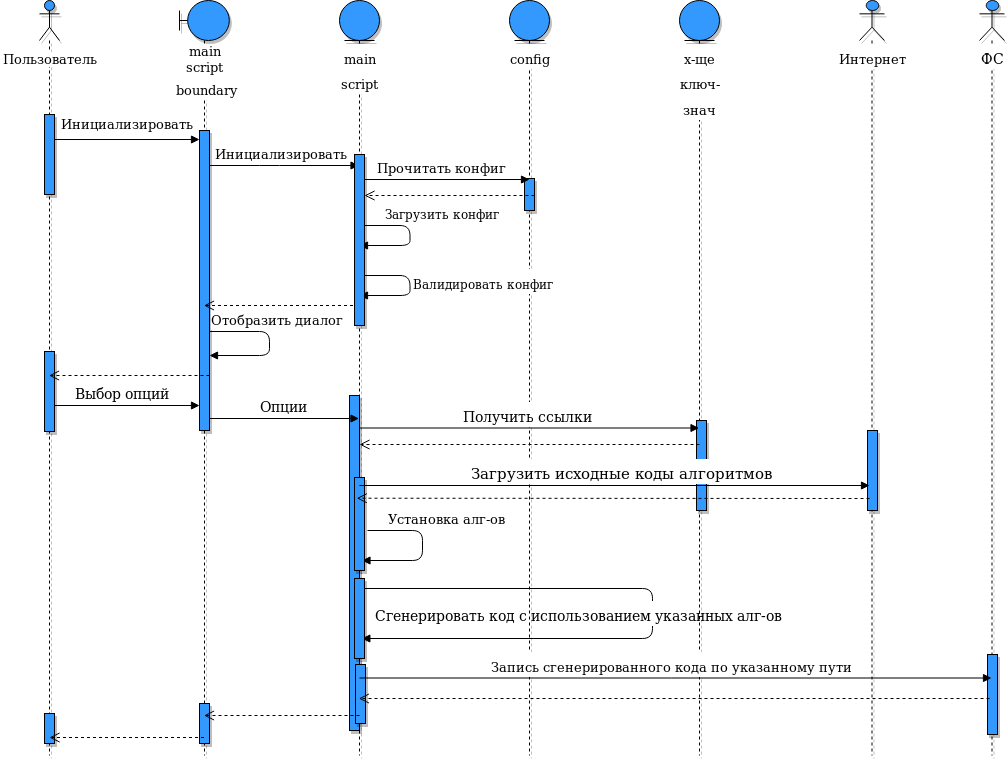
\includegraphics[width=\textwidth]{images/sequence}
    \caption{Sequence диаграмма последовательности работы первой компоненты --- компоновщика}\label{sequence}
\end{figure}

По вызову этой команды происходят процессы, обозначенные на диаграмме
последовательностей (Рис.  \ref{sequence}). Зачитывается, загружается в
программу и валидируется конфигурационный файл программы.

\newpage

Затем начинается диалог с пользователем (Рис. \ref{dialog}).
\begin{figure}[h]
    \centering
    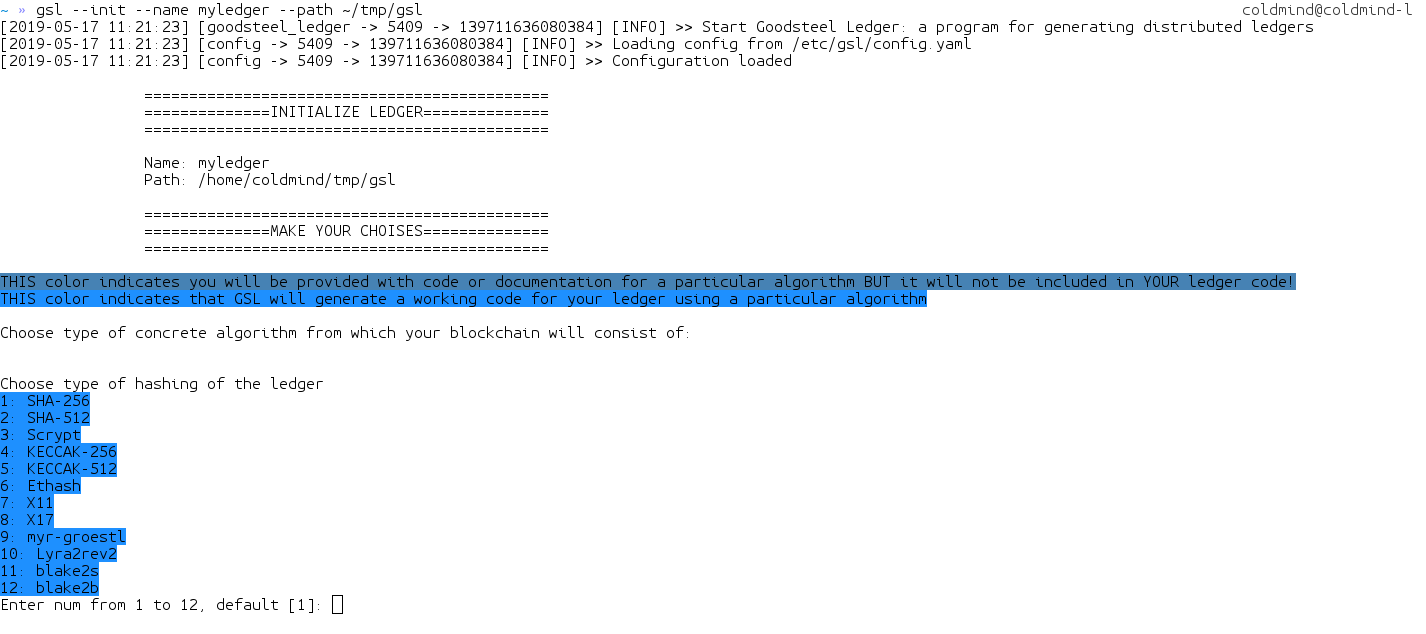
\includegraphics[width=\textwidth]{images/dialog_start}
    \caption{Начало диалога выбора алгоритмов}\label{dialog}
\end{figure}

В этом диалоге пользователь выбирает какие алгоритмы хэширования и цифровой
подписи будут использованы в его будущей реализации блокчейна. После этого,
пользователю предоставляется выбор других интересных параметров блокчейна, по
которым ему будут предложены справочные ссылки для изучения (Рис. \ref{sprav}).
После выбора происходит установка данных библиотек и генерация кода реализации
блокчейна по указанному пути (Рис. \ref{ll}).

\begin{figure}[h]
    \centering
    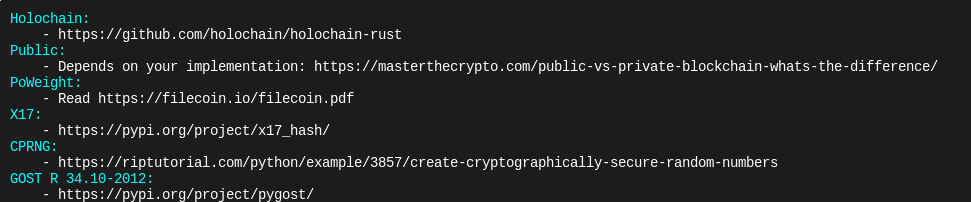
\includegraphics[width=\textwidth]{images/spravochno}
    \caption{Справочная информация по выбранным параметрам}\label{sprav}
\end{figure}

\subsubsection{Архитектура реализации блокчейна}
\begin{figure}[h]
    \centering
    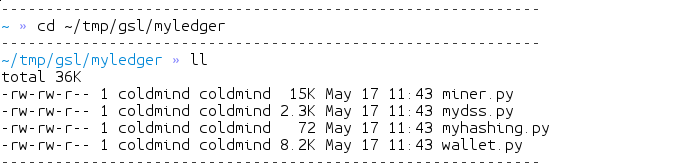
\includegraphics[width=0.8\textwidth]{images/ledger_ll}
    \caption{Директория со сгенерированным кодом реализации блокчейна}\label{ll}
\end{figure}

Код реализации блокчейна запускается интерпретатором языка Python 3.6.5.
Скрипты {\small miner.py} и {\small wallet.py} запускаются без аргументов
командной строки. Запустив {\small miner.py} (Рис. \ref{miner_run}), можно запускать {\small
wallet.py} (Рис. \ref{wallet_run}), в котором есть возможности:
\begin{enumerate}
    \item Сгенерировать кошелёк: пару публичный-приватный ключи и записать их в файл
    \item Отправить с одного кошелька на другой N условных едениц
    \item Провалидировать транзакции
\end{enumerate}

\begin{figure}[h]
    \centering
    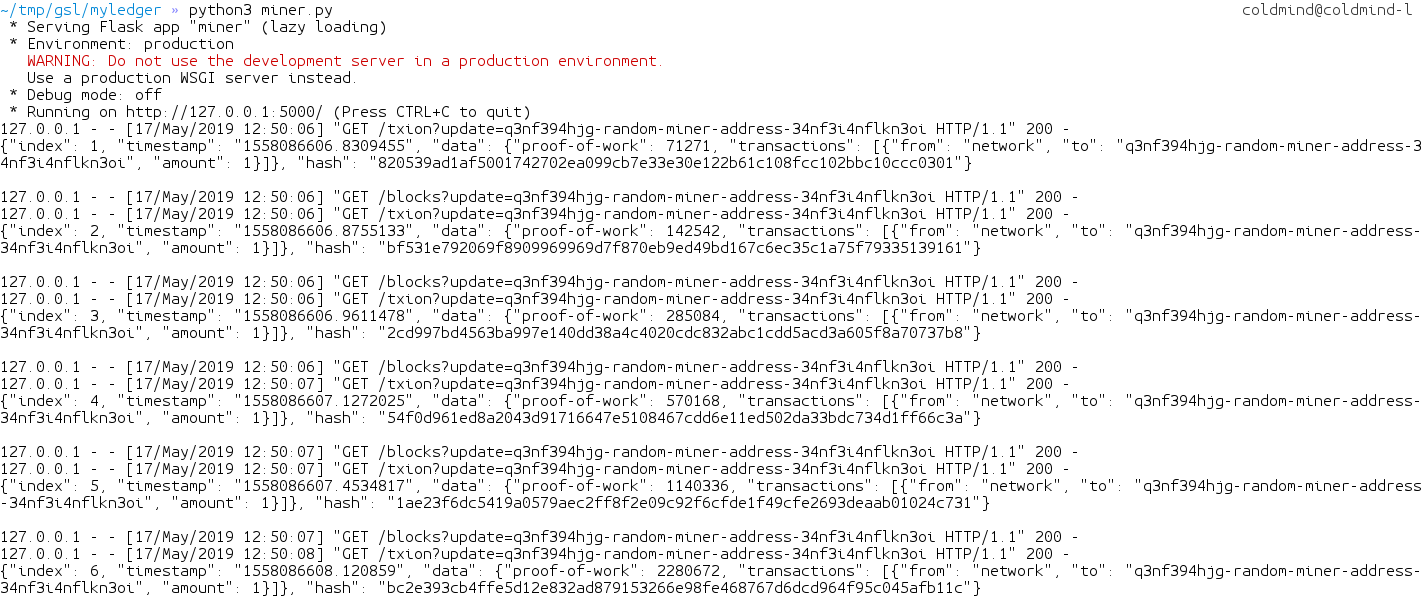
\includegraphics[width=\textwidth]{images/miner_run}
    \caption{Лог запуска майнера}\label{miner_run}
\end{figure}

\begin{figure}[h]
    \centering
    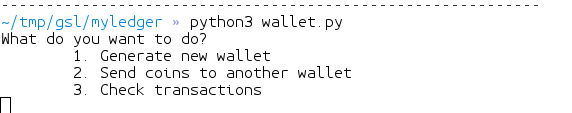
\includegraphics[width=0.8\textwidth]{images/wallet_run}
    \caption{Возможности кошелька}\label{wallet_run}
\end{figure}

Генерация пары ключей, а так же хэширование записей происходит посредством
использования выбранных ранее пользователем алгоритмов.

\newpage
\subsubsection{Работа с данными}\label{autoonova}
Исходный код алгоритмов хранится в директории {\small src/altorithms/hashing} и
{\small src/altorithms/digital\_signature}. Он собирается полным проходом в
сеть по ссылкам, расположенными в импровизированном key-value хранилище
(описано в настоящем техническом задании --- Приложение ref1). Данная процедура
происходит при автообновлении алгоритмов на сервере каждый день в 21:00
(Рис. \ref{update}). После процедуры автообновления, пользователи могут по
желанию обновить свою версию программы и использовать более свежий код.

\begin{figure}[h]
    \centering
    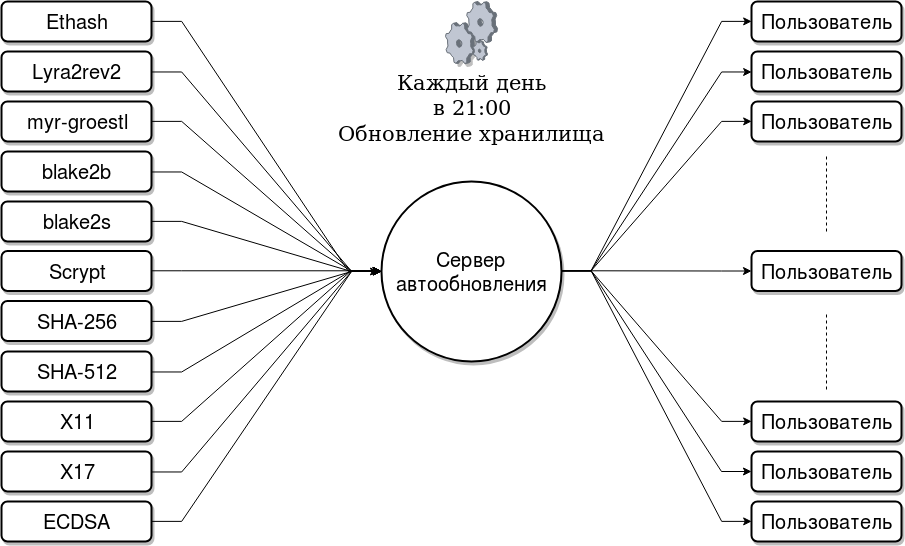
\includegraphics[width=\textwidth]{images/server}
    \caption{Процесс работы сервера автообновления}\label{update}
\end{figure}
